\documentclass[multi=tikzpicture,border=6pt]{standalone}
\usepackage{ctex}
\usepackage{amsmath}
\usepackage{tikz}
\usetikzlibrary{arrows.meta,calc,decorations.pathmorphing,patterns,positioning}
\tikzset{
  axis/.style={->,>=Stealth,thick},
  force/.style={->,>=Stealth,very thick},
  dim/.style={<->,>=Stealth,thin},
  flow/.style={->,>=Stealth,thick,blue!70!black},
  body/.style={draw=black,fill=blue!8,thick},
  nodept/.style={circle,fill=black,inner sep=1.5pt}
}
\begin{document}

% 01 question-01
\begin{tikzpicture}[x=1.2cm,y=1.2cm]
\draw[very thick] (-.4,0)--(5.15,0);\draw[very thick] (4.47214,0)--(4.47214,3.3);
\draw[blue!70!black,thick,domain=0:1.236068,samples=50] plot({2*\x},{2-\x-.5*\x*\x});
\draw[blue!70!black,thick,domain=0:1,samples=50] plot({2.472136+2*\x},{2.236068*\x-.5*\x*\x});
\draw[blue!70!black,thick,domain=1:3.236068,samples=80] plot({6.472136-2*\x},{2.236068*\x-.5*\x*\x});
\fill (0,2) circle(1.7pt) node[left]{$A$};\fill (2.472136,0) circle(1.7pt) node[below]{$B$};\fill (4.47214,1.736068) circle(1.7pt) node[right]{$C$};
\draw[flow] (0,2)--(1,1.5) node[midway,above]{$\boldsymbol v_0$};
\draw[flow] (3,.555)--(3.3,.81);\draw[flow] (2,2.47)--(1.7,2.415);
\draw[dim] (0,3.2)--(4.47214,3.2) node[midway,fill=white]{$l$};
\draw[dim] (2.472136,-.5)--(4.47214,-.5) node[midway,fill=white]{$x$};
\draw[dim] (-.65,0)--(-.65,2) node[midway,left]{$h$};
\node at (2.1,-1){质点轨迹示例：三段均满足抛体方程};
\end{tikzpicture}

% 02 solution-01
\begin{tikzpicture}[x=.9cm,y=.9cm]
\begin{scope}\draw[very thick] (-.4,0)--(5.15,0);\draw[very thick] (4.47214,0)--(4.47214,3.3);
\draw[blue!70!black,thick,domain=0:1.236068,samples=50] plot({2*\x},{2-\x-.5*\x*\x});
\draw[blue!70!black,thick,domain=0:1,samples=50] plot({2.472136+2*\x},{2.236068*\x-.5*\x*\x});
\draw[blue!70!black,thick,domain=1:3.236068,samples=80] plot({6.472136-2*\x},{2.236068*\x-.5*\x*\x});
\fill (0,2) circle(1.7pt) node[left]{$A$};\fill (2.472136,0) circle(1.7pt) node[below]{$B$};\fill (4.47214,1.736068) circle(1.7pt) node[right]{$C$};
\draw[flow] (0,2)--(1,1.5) node[midway,above]{$\boldsymbol v_0$};
\draw[flow] (3,.555)--(3.3,.81);\draw[flow] (2,2.47)--(1.7,2.415);
\node at (2,-.7){(a) 同一抛体轨迹的两次反射};\end{scope}
\begin{scope}[shift={(7,1.4)}]
\draw[very thick] (-1.8,-.6)--(1.8,-.6);\draw[fill=blue!10,thick] (0,0) circle(.6);
\draw[force,red!70!black] (0,-.6)--(0,1.2) node[left]{$J_{N1}$};
\draw[force,orange!80!black] (0,-.6)--(-1.6,-.6) node[midway,below]{$J_{f1}$};
\draw[->,thick] (.8,.4) arc(27:-65:.9) node[right]{$\omega_1<0$};
\node at (0,2){(b) 地面冲量};\end{scope}
\begin{scope}[shift={(11,1.4)}]
\draw[very thick] (.6,-1.5)--(.6,1.5);\draw[fill=blue!10,thick] (0,0) circle(.6);
\draw[force,red!70!black] (.6,0)--(-1.4,0) node[below]{$J_{N2}$};
\draw[force,orange!80!black] (.6,0)--(.6,1.3) node[right]{$J_{f2}$};
\node[align=center] at (0,-2){图示 $w_c<0$、$\sigma=+1$\\反向滑动时 $J_{f2}$ 反向};
\node at (0,2){(c) 墙面冲量};\end{scope}
\end{tikzpicture}

% 03 question-02
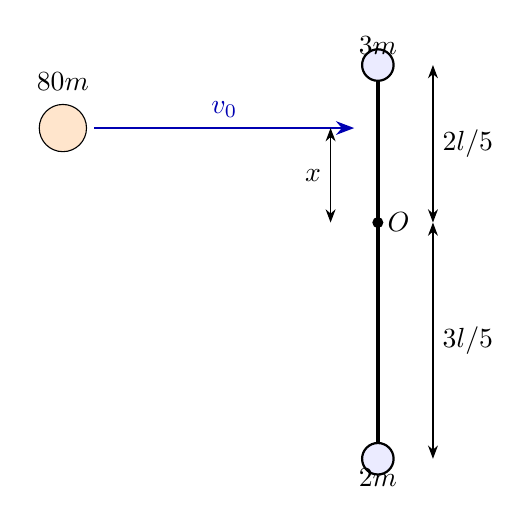
\begin{tikzpicture}[x=1cm,y=1cm]
\draw[very thick] (4,-3)--(4,2);\filldraw[body] (4,2) circle(.2) node[above]{$3m$};\filldraw[body] (4,-3) circle(.2) node[below]{$2m$};
\fill (4,0) circle(2pt) node[right]{$O$};
\draw[dim] (4.7,0)--(4.7,2) node[midway,right]{$2l/5$};\draw[dim] (4.7,-3)--(4.7,0) node[midway,right]{$3l/5$};
\draw[fill=orange!20] (0,1.2) circle(.3) node[above=.35cm]{$80m$};\draw[flow] (.4,1.2)--(3.7,1.2) node[midway,above]{$v_0$};
\draw[dim] (3.4,0)--(3.4,1.2) node[midway,left]{$x$};
\end{tikzpicture}

% 04 solution-02
\begin{tikzpicture}[x=1cm,y=1cm]
\draw[axis] (-3.5,0)--(3,0) node[right]{$X$};\draw[axis] (0,-3.4)--(0,2.8) node[above]{$Y$};
\draw[dashed] (-3,1.1)--(3,1.1) node[right]{$Y=x$};\draw[dashed] (0,-3)--(0,2);
\draw[thick] (-.8,-1.386)--(.533,.924);
\filldraw[body] (.533,.924) circle(.15) node[right]{$3m$};\filldraw[body] (-.8,-1.386) circle(.15) node[left]{$2m$};
\fill (0,0) circle(2pt) node[below right]{$O'$};
\draw[->,thick,red!70!black] (0,.85) arc(90:60:.85) node[midway,above right]{$\theta=\omega t$};
\draw[flow] (-2.2,1.1)--(-1.1,1.1) node[midway,above]{$v-V_c$（有符号）};
\node[align=center] at (0,-4.1){质心系：杆方向 $(\sin\theta,\cos\theta)$\\首次再接触须同时满足相交方程和有限杆长};
\end{tikzpicture}

% 05 question-03
\begin{tikzpicture}[scale=.9]
  % a
  \begin{scope}[shift={(0,0)}]
    \draw[thick] (0,0) circle(1.7);
    \fill (0,0) circle(2pt) node[below right]{$O$};
    \foreach \a in {90,210,330}{\draw[thick] (0,0)--(\a:1.7);}
    \node at (90:1.95){$A$};
    \node[below] at (0,-2.15){(a) 三辐条};
    \node at (.55,.25){$4r$};
    \node at (1.5,1.1){$2r$};
  \end{scope}
  % b
  \begin{scope}[shift={(5.2,0)}]
    \draw[thick] (0,0) circle(1.7);
    \fill (0,0) circle(2pt) node[below right]{$O$};
    \foreach \a in {0,45,...,315}{\draw[thick] (0,0)--(\a:1.7);}
    \node[right] at (1.7,0){$A$};
    \node[left] at (-1.7,0){$B$};
    \node at (.8,.18){$r$};
    \node at (0,.85){$4r$};
    \node[below] at (0,-2.15){(b) $2N$ 辐条};
  \end{scope}
  % c
  \begin{scope}[shift={(10.4,0)}]
    \draw[thick] (0,0) circle(1.7);
    \fill (0,0) circle(2pt) node[below right]{$O$};
    \foreach \a in {0,45,...,315}{\draw[thick] (0,0)--(\a:1.7);}
    \node[right] at (1.7,0){$A$};
    \node at (.75,.25){$4r$};
    \node at (1.5,1.05){$2r$};
    \node[below] at (0,-2.15){(c) $N$ 辐条};
  \end{scope}
\end{tikzpicture}

% 06 solution-03
\begin{tikzpicture}[x=1cm,y=1cm]
\tikzset{res/.style={decorate,decoration={zigzag,segment length=4pt,amplitude=2pt}}}
\begin{scope}
\foreach \i in {0,...,4}{\fill (1.8*\i,0) circle(1.5pt);\draw[thick] (1.8*\i,0)--(1.8*\i,-.3);\draw[thick,res] (1.8*\i,-.3)--(1.8*\i,-1.2);\draw[thick] (1.8*\i,-1.2)--(1.8*\i,-1.5);}
\foreach \i in {0,...,3}{\draw[thick] (1.8*\i,0)--(1.8*\i+.3,0);\draw[thick,res] (1.8*\i+.3,0)--(1.8*\i+1.5,0);\draw[thick] (1.8*\i+1.5,0)--(1.8*\i+1.8,0);\node[above] at (1.8*\i+.9,.05){$r$};}
\draw[thick] (0,-1.5)--(7.2,-1.5) node[right]{$O$};\node[above left] at (0,0){$A$};\node[above right] at (7.2,0){$B$};
\node[left] at (0,-.75){$r$};\node[right] at (7.2,-.75){$r$};\foreach \i in {1,2,3}{\node[right] at (1.8*\i,-.75){$2r$};}
\node at (3.6,.8){(a) 第（2）问折叠后的梯形网络};\end{scope}
\begin{scope}[shift={(0,-3.8)}]
\foreach \i in {0,...,4}{\fill (1.8*\i,0) circle(1.5pt);\ifnum\i=4\node[above] at (1.8*\i,.05){$U_N$};\else\node[above] at (1.8*\i,.05){$U_{\i}$};\fi\draw[thick] (1.8*\i,0)--(1.8*\i,-.3);\draw[thick,res] (1.8*\i,-.3)--(1.8*\i,-1.2);\draw[thick] (1.8*\i,-1.2)--(1.8*\i,-1.5);\node[right] at (1.8*\i,-.75){$4r$};}
\foreach \i in {0,...,3}{\draw[thick,res] (1.8*\i,0)--(1.8*\i+1.8,0);\node[below] at (1.8*\i+.9,0){$2r$};}
\draw[thick] (0,-1.5)--(7.2,-1.5) node[right]{$O$};
\node[align=center] at (3.6,-2.25){(b) 第（3）问的周期链（省略中间节点）\\左右端同为 $A$：$U_N=U_0$，两端辐条只计一次};
\node at (3.6,.85){$2U_{i-1}-5U_i+2U_{i+1}=0$};
\end{scope}\end{tikzpicture}

% 07 question-04
\begin{tikzpicture}[x=1cm,y=1cm]
  % stylized aircraft
  \begin{scope}[shift={(0,0)}]
    \draw[fill=blue!8,thick]
      (0,1.45)--(1.45,1.25)--(2.1,.2)--(2.45,.2)--(2.2,1.35)
      --(3.8,1.75)--(3.8,2.05)--(2.2,2.45)--(2.45,3.55)
      --(2.1,3.55)--(1.45,2.5)--(0,2.3)--cycle;
    \draw[thick] (1.55,1.25)--(1.55,2.5);
    \draw[thick] (1.85,1.3)--(1.85,2.45);
    \node at (1.9,-.2){(a) 无转动结构离子风飞机示意};
  \end{scope}
  % emitter–collector assembly
  \begin{scope}[shift={(5.0,.45)}]
  \draw[fill=gray!12,thick,rounded corners] (.2,.4)--(2.1,.4)--(2.7,1.15)--(5.7,1.15)--(6.25,.4)--(8.4,.4)--(8.4,1.35)--(.2,1.35)--cycle;
  \draw[very thick] (1.1,1.35)--(1.1,2.35)--(1.35,2.35)--(1.35,1.35);
  \draw[very thick] (7.1,1.35)--(7.1,2.05)--(7.45,2.05)--(7.45,1.35);
  \node[above] at (1.25,2.35){发射电极};
  \node[above] at (7.28,2.05){收集电极};
  \foreach \y in {1.55,1.75,1.95}{
    \draw[flow] (1.4,\y)--(6.95,\y);
  }
  \foreach \x in {2.0,3.0,4.0,5.0,6.0}{\fill[blue!70!black] (\x,1.75) circle(1.7pt);}
  \node[blue!70!black] at (4.2,2.25){$\mathrm{N_2^+}$ 离子流};
  \draw[dim] (1.25,.05)--(7.28,.05) node[midway,fill=white]{$l$};
  \node at (4.2,-.35){(b) 发射—收集电极组件};
  \end{scope}
\end{tikzpicture}

% 08 solution-04
\begin{tikzpicture}[x=.8cm,y=.8cm]
\draw[axis] (0,0)--(10.5,0) node[right]{$s$};\draw[axis] (0,0)--(0,3.8) node[above]{$v$};
\foreach \i in {0,...,4}{\draw[blue!70!black,thick,domain=0:2,samples=65] plot({2*\i+\x},{2.8*sqrt(\x/2)});\draw[red!70!black,dashed] (2*\i+2,2.8)--(2*\i+2,0);}
\draw[dim] (0,-.55)--(2,-.55) node[midway,below=1pt]{$\lambda$};
\node at (5,4.3){$v=\sqrt{2(eU/ml)(s-s_i)}$};\node at (5,-1.2){每次碰撞后速度归零};
\end{tikzpicture}

% 09 question-05
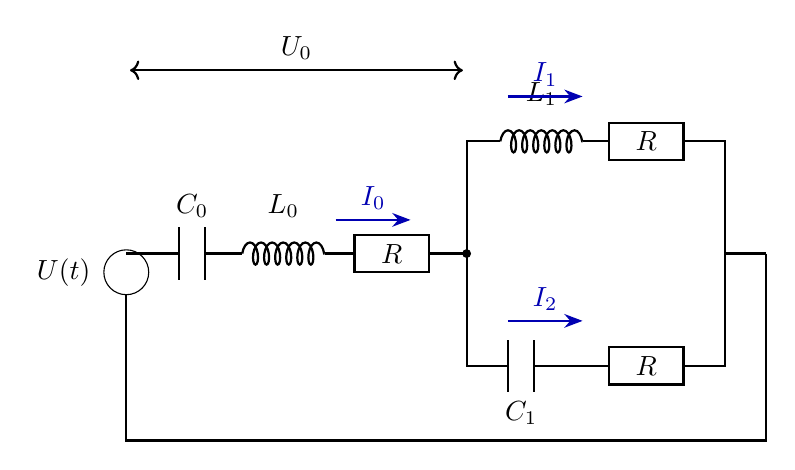
\begin{tikzpicture}[x=.95cm,y=.95cm]
  \draw[thick] (0,0)--(.7,0);
  \draw[thick] (.7,-.35)--(.7,.35);
  \draw[thick] (1.05,-.35)--(1.05,.35);
  \node[above] at (.88,.35){$C_0$};
  \draw[thick] (1.05,0)--(1.55,0);
  \draw[thick,decorate,decoration={coil,aspect=.45,segment length=4pt,amplitude=4pt}] (1.55,0)--(2.65,0);
  \node[above] at (2.1,.35){$L_0$};
  \draw[thick] (2.65,0)--(3.05,0);
  \draw[thick] (3.05,-.25) rectangle (4.05,.25);
  \node at (3.55,0){$R$};
  \draw[thick] (4.05,0)--(4.55,0);
  \fill (4.55,0) circle(1.6pt);
  \draw[thick] (4.55,0)--(4.55,1.5)--(5,1.5);
  \draw[thick,decorate,decoration={coil,aspect=.45,segment length=4pt,amplitude=4pt}] (5,1.5)--(6.1,1.5);
  \node[above] at (5.55,1.85){$L_1$};
  \draw[thick] (6.1,1.5)--(6.45,1.5);
  \draw[thick] (6.45,1.25) rectangle (7.45,1.75);
  \node at (6.95,1.5){$R$};
  \draw[thick] (7.45,1.5)--(8,1.5)--(8,0);
  \draw[thick] (4.55,0)--(4.55,-1.5)--(5.1,-1.5);
  \draw[thick] (5.1,-1.85)--(5.1,-1.15);
  \draw[thick] (5.45,-1.85)--(5.45,-1.15);
  \node[below] at (5.28,-1.85){$C_1$};
  \draw[thick] (5.45,-1.5)--(6.45,-1.5);
  \draw[thick] (6.45,-1.75) rectangle (7.45,-1.25);
  \node at (6.95,-1.5){$R$};
  \draw[thick] (7.45,-1.5)--(8,-1.5)--(8,0);
  \draw[thick] (8,0)--(8.55,0);
  \draw[thick] (8.55,0)--(8.55,-2.5)--(0,-2.5)--(0,-.55);
  \draw (0,-.25) circle(.3);
  \node[left] at (-.35,-.25){$U(t)$};
  \draw[<->,thick] (.05,2.45)--(4.5,2.45) node[midway,above]{$U_0$};
  \draw[flow] (2.8,.45)--(3.8,.45) node[midway,above]{$I_0$};
  \draw[flow] (5.1,2.1)--(6.1,2.1) node[midway,above]{$I_1$};
  \draw[flow] (5.1,-.9)--(6.1,-.9) node[midway,above]{$I_2$};
\end{tikzpicture}

% 10 solution-05
\begin{tikzpicture}[x=1cm,y=1cm]
  \draw[axis] (-.2,0)--(6,0) node[right]{$\operatorname{Re}$};
  \draw[axis] (0,-2.4)--(0,2.4) node[above]{$\operatorname{Im}$};
  \draw[force,blue!70!black] (0,0)--(4.6,0) node[below right]{$\boldsymbol I_0$};
  \draw[force,orange!80!black] (0,0)--(2.3,1.65) node[above]{$\boldsymbol I_2$};
  \draw[force,red!70!black] (0,0)--(2.3,-1.65) node[below]{$\boldsymbol I_1$};
  \draw[dashed] (2.3,1.65)--(4.6,0)--(2.3,-1.65);
  \draw[->] (1.1,0) arc[start angle=0,end angle=35.7,radius=1.1] node[midway,right]{$\varphi$};
  \draw[->] (1.35,0) arc[start angle=0,end angle=-35.7,radius=1.35] node[midway,right]{$\varphi$};
  \node[align=center] at (3.3,2.35){并联两支路的电流相位\\关于总电流对称};
\end{tikzpicture}

% 11 question-06
\begin{tikzpicture}[x=1cm,y=1cm]
  \draw[very thick] (0,0) rectangle (4.5,4.5);
  \node[left] at (0,2.25){板 1：$T_1$};
  \node[above] at (2.25,4.5){板 2：$T_2$};
  \node[right] at (4.5,2.25){板 3：$T_3$};
  \node[below] at (2.25,0){板 4：$T_4$};
  \fill (1.5,0) circle(2pt) node[below=.35cm]{$P$};
  \draw[dim] (0,-.75)--(1.5,-.75) node[midway,fill=white]{$x$};
  \draw[dim] (1.5,-.75)--(4.5,-.75) node[midway,fill=white]{$l-x$};
  \draw[dashed] (1.5,0)--(0,4.5);
  \draw[dashed] (1.5,0)--(4.5,4.5);
  \draw[dim] (5.05,0)--(5.05,4.5) node[midway,right]{$l$};
\end{tikzpicture}

% 12 solution-06
\begin{tikzpicture}[x=.88cm,y=.88cm]
  % 左侧：正方形截面内的点到面元几何
  \begin{scope}
    \draw[very thick] (0,0) rectangle (5,5);
    \coordinate (P) at (1.6,0);
    \coordinate (D1) at (0,3.35);
    \coordinate (D2) at (3.55,5);
    \coordinate (D3) at (5,2.75);
    \fill (P) circle(2pt) node[below=.12cm]{$P$};
    \draw[red!75!black,very thick] ($(D1)+(0,-.28)$)--($(D1)+(0,.28)$);
    \draw[red!75!black,very thick] ($(D2)+(-.28,0)$)--($(D2)+(.28,0)$);
    \draw[red!75!black,very thick] ($(D3)+(0,-.28)$)--($(D3)+(0,.28)$);
    \node[left] at (D1){$\mathrm dA_1$};
    \node[above] at (D2){$\mathrm dA_2$};
    \node[right] at (D3){$\mathrm dA_3$};
    \draw[flow] (P)--(D1) node[midway,left]{$\rho_1$};
    \draw[flow] (P)--(D2) node[midway,left]{$\rho_2$};
    \draw[flow] (P)--(D3) node[midway,right]{$\rho_3$};
    \draw[dashed] (P)--++(0,3.7) node[above]{$\boldsymbol n_s$};
    \draw[dashed] (D1)--++(1.25,0) node[right]{$\boldsymbol n_1$};
    \draw[dashed] (D2)--++(0,-1.15) node[below]{$\boldsymbol n_2$};
    \draw[dashed] (D3)--++(-1.15,0) node[left]{$\boldsymbol n_3$};
    \draw[dim] (0,-.65)--(1.6,-.65) node[midway,fill=white]{$x$};
    \draw[dim] (1.6,-.65)--(5,-.65) node[midway,fill=white]{$l-x$};
    \draw[dim] (-.65,0)--(-.65,3.35) node[midway,fill=white]{$y$};
    \draw[dim] (0,5.65)--(3.55,5.65) node[midway,fill=white]{$\xi$};
    \node at (2.5,-1.15){横截面内的投影几何};
  \end{scope}

  % 右侧：轴向间隔为何进入 R^2
  \begin{scope}[shift={(7.0,1.0)}]
    \node[font=\bfseries] at (1.8,4.05){轴向积分};
    \coordinate (S) at (0,.4);
    \coordinate (Q) at (3.25,3.0);
    \coordinate (Qp) at (3.25,.4);
    \fill (S) circle(2pt) node[left]{$P$};
    \fill (Q) circle(2pt) node[right]{$\mathrm dA$};
    \draw[flow] (S)--(Q) node[midway,above left]{$R$};
    \draw[dashed] (S)--(Qp) node[midway,below]{$\rho$};
    \draw[dashed] (Qp)--(Q) node[midway,right]{$z$};
    \draw (2.92,.4) rectangle (3.25,.73);
    \node[align=left] at (1.7,-.45){$R^2=\rho^2+z^2$\\[2pt]
      $\displaystyle \mathrm dq\propto
      \frac{\cos\theta_s\cos\theta_r}{R^2}\,\mathrm dA$};
  \end{scope}
\end{tikzpicture}

% 13 question-07
\begin{tikzpicture}[x=1cm,y=1cm]
\draw[dashed] (-.8,0)--(9.2,0);
\foreach \x/\lab in {0/样品,4/傅里叶面,8/像面}{\draw[thick] (\x,-1.4)--(\x,1.4);\node[above] at (\x,1.5){\lab};}
\foreach \x/\lab in {2/L_1,6/L_2}{\draw[thick] (\x,0) ellipse(.15 and 1.3);\node[above] at (\x,1.5){$\lab$};}
\foreach \x in {0,2,4,6}{\draw[dim] (\x,-1.8)--(\x+2,-1.8) node[midway,fill=white]{$f$};}
\foreach \h in {-.9,0,.9}{\draw[flow] (-.7,\h)--(2,\h)--(4,0)--(6,-\h)--(8,-\h);}
\fill[red!70!black] (4,0) circle(3pt);\fill[blue!70!black] (4,.7) circle(2pt);\fill[blue!70!black] (4,-.7) circle(2pt);
\node at (4,-2.5){图示零级平面波光路；像坐标发生倒置};
\end{tikzpicture}

% 14 solution-07
\begin{tikzpicture}[x=1cm,y=1cm]
\draw[axis] (-4.5,0)--(4.5,0) node[right]{$k_x$};
\draw[force,blue!70!black] (0,0)--(0,2.5);\node[above] at (0,2.5){$A(1+i\varphi_0/2)$};\node[below] at (0,0){$0$};
\foreach \x/\lab in {-3/-k_*,3/k_*}{\draw[force,blue!70!black] (\x,0)--(\x,1.25);\node[below] at (\x,0){$\lab$};\node[above] at (\x,1.25){$iA\varphi_0/4$};}
\node[align=center] at (0,-1.25){零级 $\times1/4$；非零级 $\times i$\\箭头高度仅示意频谱，标注为复振幅系数};
\end{tikzpicture}

% 15 solution-08
\begin{tikzpicture}[x=1cm,y=1cm]
  \foreach \x/\lab/\p in {0/{1}/{p_1},3/{2}/{p_2},6/{3}/{p_3}}{
    \draw[fill=blue!10,thick] (\x,0) circle(.55);
    \node at (\x,0){$\lab$};
    \node[below=.6cm] at (\x,0){$\p$};
  }
  \draw[flow,bend left=18] (0.5,.2) to node[above]{$v_{12}p_1$} (2.5,.2);
  \draw[flow,bend left=18] (2.5,-.2) to node[below]{$v_{12}p_2$} (.5,-.2);
  \draw[flow,bend left=18] (3.5,.2) to node[above]{$v_{23}p_2$} (5.5,.2);
  \draw[flow,bend left=18] (5.5,-.2) to node[below]{$v_{23}p_3$} (3.5,-.2);
  \node[align=center] at (3,2){跃迁系数对称不等于概率流相等\\净流由概率差决定，并使 $H$ 单调不增};
\end{tikzpicture}

\end{document}
